\documentclass{standalone}
\usepackage{tikz}

\begin{document}

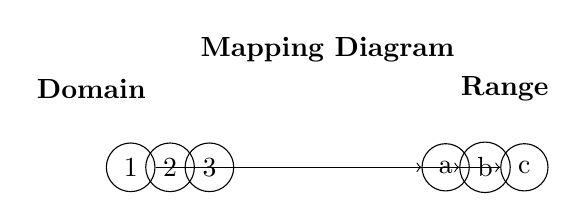
\begin{tikzpicture}
    % Title for the diagram
    \node at (2.5, 1.5) {\textbf{Mapping Diagram}};
    
    % Domain nodes (close together, circular shapes)
    \node[circle, draw, minimum size=0.6cm] (d1) at (0, 0) {1};
    \node[circle, draw, minimum size=0.6cm] (d2) at (0.5, 0) {2};
    \node[circle, draw, minimum size=0.6cm] (d3) at (1, 0) {3};
    
    % Range nodes (close together, circular shapes)
    \node[circle, draw, minimum size=0.6cm] (r1) at (4, 0) {a};
    \node[circle, draw, minimum size=0.6cm] (r2) at (4.5, 0) {b};
    \node[circle, draw, minimum size=0.6cm] (r3) at (5, 0) {c};
    
    % Draw skew arrows (bent left for slant)
    \draw[->, bend left=30] (d1) -- (r1);
    \draw[->, bend left=30] (d2) -- (r2);
    \draw[->, bend left=30] (d3) -- (r3);
    
    % Label domain and range (clear titles above nodes)
    \node at (-0.5, 1) {\textbf{Domain}}; % Above domain nodes
    \node at (4.75, 1) {\textbf{Range}};  % Above range nodes
\end{tikzpicture}

\end{document}